\chapter{Περιγραφή του Προβλήματος}
\label{ch:chapter1}
Ζητούμενο της παρούσας εργασίας ήταν η υλοποίηση μεθόδων στο περιβάλλον \selectlanguage{english}
Matlab,\selectlanguage{greek} για την εύρεση ελαχίστου τριών συναρτήσεων σε δεδομένο διάστημα και η μελέτη του πλήθους υπολογισμών που απαιτεί η κάθε μία σε μεταβαλλόμενες συνθήκες. 
\section{Οι Μέθοδοι}
Οι μέθοδοι προς υλοποίηση είναι οι εξής:
\begin{itemize}
    \item Μέθοδος Διχοτόμου
    \item Μέθοδος Χρυσού Τομέα
    \item Μέθοδος $Fibonacci$
    \item Μέθοδος Διχοτόμου με χρήση παραγώγων
\end{itemize}

\section{Η Μελέτη}
Οι συναρτήσεις προς ελαχιστοποίηση είναι οι παρακάτω :
\begin{itemize}
    \item $f1 = (x - 2)^2 + x \log(x + 3)$
    \item $f2 =  e^{-2x} + (x - 2)^2$
    \item $f3 = e^x(x^3 - 1) + (x - 1)\sin(x)$
\end{itemize}

\begin{figure}[H]
    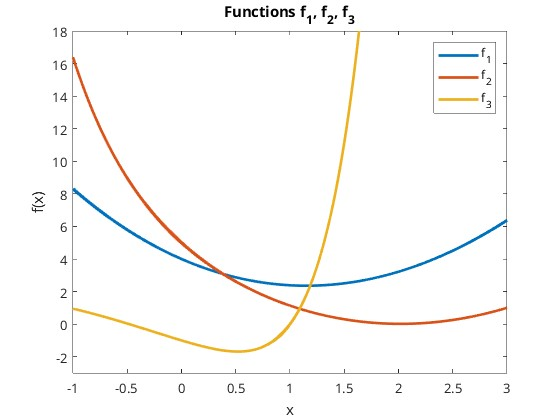
\includegraphics[scale=0.7]{plots/prereqs/funcs.jpg}
    \label{fig:funcs}
    \caption{Οι συναρτήσεις προς ελαχιστοποίηση}
    \centering
\end{figure}

Για κάθε μία εκ των παραπάνω συναρτήσεων, καλούμαστε στο διάστημα $[a_0, b_0] = [-1 , 3]$ να αναζητήσουμε
το ελάχιστο τους, χρησιμοποιώντας της παραπάνω μεθόδους. Τη συγκεκριμένη διαδικασία την επαναλαμβάνουμε για διαφορετικές τιμές του $l$, ενώ στην περίπτωση της
Μεθόδου Διχοτόμου χωρίς παραγώγους μεταβάλλουμε και το $e$. Κάθε φορά που καλείται κάποια συνάρτηση θα καταγράφονται οι υπολογισμοί που χρειάστηκε να εκτελέσει η $f_i(x)$ για σκοπούς ανάλυσης.